\documentclass[12pt]{article}

\usepackage[fleqn]{amsmath}
\usepackage{amssymb}
\usepackage{amsthm}
\usepackage{graphicx}
\usepackage{float}
\theoremstyle{plain}     %------- 'regular' theorem types
\newtheorem{thm}{Theorem}[section]
\newtheorem{cor}[thm]{Corollary}
\newtheorem{lemma}[thm]{Lemma}
\newtheorem{prop}[thm]{Proposition}
\newtheorem{example}[thm]{Example}
\newtheorem{exer}[thm]{Exercise}
\newtheorem{define}[thm]{Definition}
\usepackage[top=2cm, left=2cm, right=2cm]{geometry} 
\usepackage{parskip}
\setlength{\parindent}{0in}
\usepackage{floatflt}
\usepackage{multicol}
\usepackage{tabu}
\usepackage[hidelinks]{hyperref}
\hypersetup{
	urlcolor=blue}

%%%%%%%%%%%%%%%%%%%%%%
%%%%%%%%%%%%%%%%%%%%%%%
%%%%%%%%%%%%%%%%%%%%%%%%
\begin{document}
\large
%subject
City Semester  %\hspace{8cm} Name:\makebox[6cm]{\hrulefill}
\\
%specific topic
NYC biome\\
\normalsize 
%\emph{Complete all work on a separate sheet of paper with exercises clearly labeled and all reasoning and work given.}\\[.5cm]
\emph{Show all work for full credit.}\\
One method of classifying biomes is by the amount of rainfall per year and the average annual temperature as shown in the figure below.
	\begin{figure}[H]
		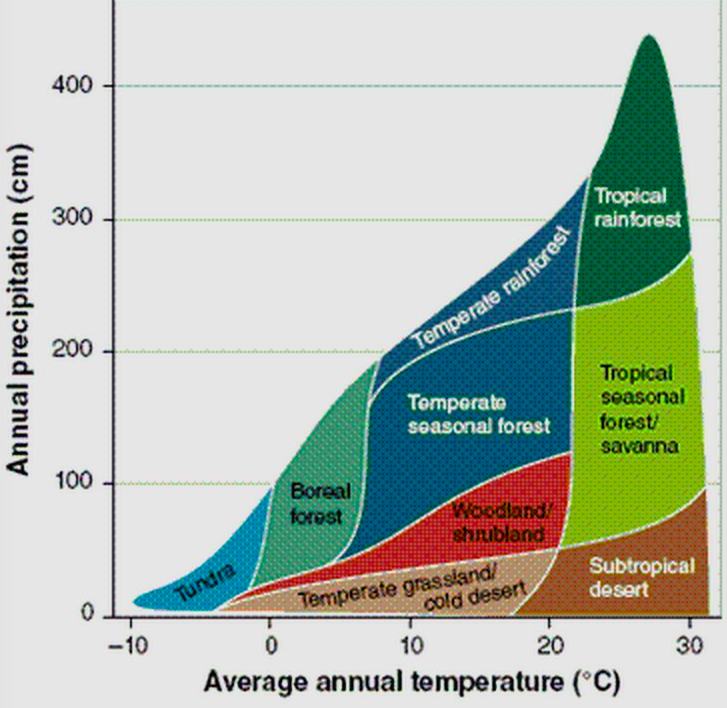
\includegraphics[scale=.5]{a.png}
	\end{figure}
\begin{enumerate}
	\item Use Fathom to obtain the five number summary for annual precipitation in centimeters. Create a boxplot for this data and describe the distribution.\\
	\item Use Fathom to obtain the five number summary of the annual average temperature in Celsius. Create a boxplot for this data and describe the distribution.\\
	\item Classify NYC as one of the biome's in the above figure.\\
	\item Plot the average annual temperature over time as a line graph. Is it what you expected?\\
	\item Observe something interesting about the data set you have.
\end{enumerate}
	
\end{document} 